Recent work has begun to expand diffusion language models (DLLMs) beyond pure text generation into the realms of multimodal understanding and complex reasoning. In the multimodal domain, Diffusion Language Models Can Perform Many Tasks with Scaling and Instruction-Finetuning demonstrates that a single discrete-diffusion backbone can be extended to process image inputs and answer visual questions. By following the two-phase training paradigm of LLaVA—first interleaving visual and textual encodings in a frozen vision encoder, then instruction-fine-tuning the diffusion decoder—DLLMs attain zero-shot performance on vision-language benchmarks without specialized cross-modal architectures \cite{ye_diffusion_2025}. This result highlights DLLMs’ ability to treat images as another “language” of tokens, leveraging the random-masking denoising process to fuse visual and linguistic representations seamlessly.

On the reasoning front, \textbf{d1: Scaling Reasoning in Diffusion Large Language Models via Reinforcement Learning} introduces a two-stage post-training framework—supervised fine-tuning on high-quality reasoning traces followed by a novel policy gradient method (\textbf{diffu-GRPO})—to imbue masked DLLMs with stepwise planning capabilities. Remarkably, as sequence lengths exceed 512 tokens, the model begins to exhibit self-correction and backtracking behaviors, mirroring the “chain-of-thought” processes seen in autoregressive counterparts, yet without relying on a fixed generation order. Furthermore, instruction-fine-tuned DLLMs are shown to conform their generative steps to a topological sort of the underlying causal graph—first generating premises, then formulas, then conclusions—underscoring their inherent advantage in modeling non-linear dependencies over unidirectional AR decoders \cite{zhao_d1_2025}.

The key innovation of \textbf{d1} lies in adapting Group Relative Policy Optimization (GRPO) for the DLLM's architecture. Traditional policy gradient methods encounter challenges here due to DLLMs non-autoregressive nature. To address this, the authors develop diffu-GRPO, which modifies the standard GRPO objective to handle partially masked sequences. To compute the log-probability of each token $o$ in the sequence in the diffu-GRPO framework, for a given prompt $q$, a perturb process is executed on it where each token randomly gets masked with probability $p_{\text{mask}}$, generating a masked prompt $q'$. Then a one step unmasking process is executed to obtain the estimation of per-token log-probability $\log \pi_\theta(o^k | q)$, $1\leq k \leq |o|$. The advantage for token $k$ in response $o_i$ is computed using the group-relative approach: 
\begin{equation}
A_i^k(\pi) = r_i(\pi) - \text{mean}\left(\{r_j(\pi)\}_{j=1}^G\right), \quad 1 \leq k \leq |o_i|,
\label{eq:grpo-advantage}
\end{equation}%
where $r_i(\pi)$ represents the reward for response $i$, and $G$ is the total number of responses sampled from the current policy. The optimization objective combines this advantage calculation with policy gradient updates specifically designed for masked sequences. The diffu-GRPO loss function incorporates both the policy improvement term and KL divergence regularization:
\begin{equation}
\begin{aligned}
\mathcal{L}_{\text{diffu-GRPO}}(\theta) &= \mathbb{E}_{\substack{q \sim \mathcal{D},\, q' \sim \text{masking}(q),\\
              o_1,\dots,o_G \sim \pi_{\theta_{\text{old}}}(\,\cdot \mid q)}}\Bigg[
\frac{1}{G}\sum_{i=1}^{G}\frac{1}{|o_i|}\sum_{k=1}^{|o_i|}\\
&\quad\min\!\Bigg(
      \frac{\phi^{\pi_\theta}(o^k_i \mid q')}
           {\phi^{\pi_{\theta_{\text{old}}}}(o^k_i \mid q')}A_i^{k},\\
&\qquad\operatorname{clip}\!\Bigg(
        \frac{\phi^{\pi_\theta}(o^k_i \mid q')}
             {\phi^{\pi_{\theta_{\text{old}}}}(o^k_i \mid q')},
        1-\varepsilon,\,1+\varepsilon
  \Bigg)A_i^{k}
\Bigg)\\
&\quad-\beta\,D_{\text{KL}}\!\Bigl[
   \phi^{\pi_\theta}(\cdot \mid q')\,\bigl\|\,\phi^{\pi_{\text{ref}}}(\cdot \mid q')
\Bigr]
\Bigg],
\end{aligned}
\label{eq:diffugrpo}
\end{equation}%
where $\phi^{\pi_\theta}(o^k \mid q')$ and $\phi^{\pi_\theta}(o \mid q')$  denote the estimated per-token and sequence probabilities for $\pi_\theta$, and $\beta$ controls the strength of the KL divergence penalty. The algorithm of diffu-GRPO is summarized in Algorithm~\ref{alg:diffu-grpo}.

\begin{algorithm}[H]
\footnotesize
\caption{diffu-GRPO: Policy Gradient Optimization for Masked dLLMs (Reproduced from d1~\cite{zhao_d1_2025})}
\label{alg:diffu-grpo}
\begin{algorithmic}[1]
\State \textbf{Require:} Reference model $\pi_{\text{ref}}$, prompt distribution $\mathcal{D}$, number of completions per prompt $G$, number of inner updates $\mu$, prompt token masking probability $p_{\text{mask}}$
\State \textbf{Initialize} $\pi_\theta \leftarrow \pi_{\text{ref}}$
\While{not converged}
    \State $\pi_{\text{old}} \leftarrow \pi_\theta$
    \State Sample a prompt $q \sim \mathcal{D}$
    \State Sample $G$ completions $o_i \sim \pi_{\theta_{\text{old}}}(\cdot | q)$, $i \in [G]$\
    \State For each $o_i$, compute reward $r_i$ and advantage $A_i^k(\pi_{\theta_{\text{old}}})$ using Eq.~\ref{eq:grpo-advantage}
    \For{gradient update iterations $n = 1, \ldots, \mu$}
        \State $q' \leftarrow$ randomly mask tokens of prompt $p$ with probability $p_{\text{mask}}$
        \State For $\pi_\theta, \pi_{\theta_{\text{old}}}, \pi_{\text{ref}}$, estimate log-probabilities of $o_i$ given $q'$ 
        \State Compute diffu-GRPO objective (\ref{eq:diffugrpo}) and update $\pi_\theta$ by gradient descent
    \EndFor
\EndWhile
\State \Return $\pi_\theta$
\end{algorithmic}
\end{algorithm}

By abstracting both images and complex logical steps as masked tokens in a unified diffusion process, these frontier studies reveal that DLLMs can serve as generalist engines for multimodal perception and multi-step reasoning. Future work will undoubtedly refine these training recipes and explore more modality integrations and "knowledge transfer" of different modalities between AR models and DLLMs.

\begin{figure*}[ht]
    {\centering
    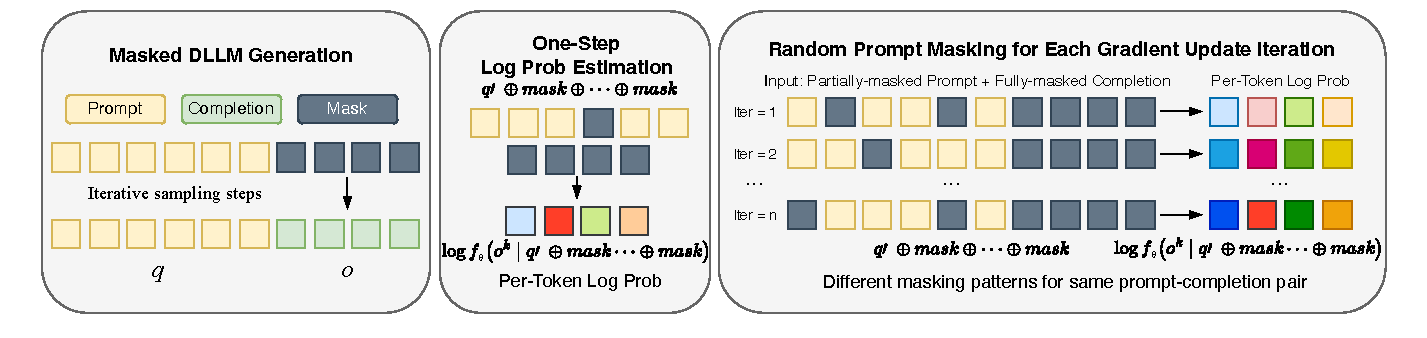
\includegraphics[width=1.0\textwidth]{"figs/d1_Scaling_Reasoning/diffu-GRPO.pdf"}
    \par}
    \caption{\textbf{Log Probability Estimation in diffu-GRPO.} First the completion $o$ is generated from prompt $q$ using full diffusion sampling \textbf{(left)}. Then token-level log probabilities are computed using a single forward pass for each masking pattern \textbf{(mid)}. The log-probability from one-step unmasking is used as the estimation method. During policy gradient updates, a random masking pattern is applied to the prompt to create $q'$, while the completion stays fully masked \textbf{(right)}. The color gradients in per-token log probabilities show that different masking patterns give different estimates of token-level log probabilities. This works as a regularization method for policy optimization, allowing more gradient updates per batch. This approach reduces the number of online generations needed for RL training.}
    \label{fig:diffu-GRPO}
\end{figure*}

% \bibliographystyle{plain}
% \bibliography{DLLM}
